\documentclass{report}


\usepackage{bibgerm}
\usepackage[numbers,sort&compress]{natbib}
\usepackage{amsmath,amssymb,mathtools}
\usepackage{algpseudocode,algorithm}
\usepackage{graphicx}
\usepackage{hyperref}
\usepackage{multirow}
\usepackage[utf8]{inputenc}
\usepackage{geometry}
\usepackage{parskip}
\usepackage{paralist}
\usepackage{multicol}

\geometry{verbose,a4paper,tmargin=25mm,bmargin=25mm,lmargin=15mm,rmargin=20mm}

%% Stuff ist aus ML1. vllt brauchen wir es ja noch :D
\DeclareMathOperator*{\argmax}{arg\,max}
\DeclareMathOperator*{\argmin}{arg\,min}

\newcommand{\IndState}[1][1]{\State\hspace{10mm}}
\newcommand{\mparagraph}[1]{\paragraph{#1} \mbox{}\\}

%%%%%%%%%%%%%% includeonly %%%%%%%%%%%%%%%%%%%
% Es werden nur die Teile eingebunden, die hier
% aufgefuehrt sind!
%\include{Kapitel X}
%}um es anzuzeigen.
%%%%%%%%%%%%%%%%%%%%%%%%%%%%%%%%%%%%%%%%%%%%%%
\graphicspath{{pic/}}

\begin{document}

\tableofcontents


% einfach !TEX root = rob1.tex an den Anfang packen von chaptern
% !TEX root = rob1.tex
\chapter{Einführung}

\subsection{Begriffsbildung}

\mparagraph{Roboter}
\begin{compactitem}
    \item \textbf{Industrie}: Ein Roboter ist ein frei programmierbarer, multifunktionaler
    Manipulator mit mindenstes 3 unabhängigen Achsen, um Materialien, Teile, Werkzeuge oder
    Geräte auf programmierten, variablen Bahnen zu bewegen zur Erfüllung verschiedener Aufgaben.
    \item \textbf{Wissenschaft}: Roboter sind sensomotorische Maschinen zur Erweiterung der
    menschlichen Handlungsfähigkeit. Sie bestehen aus mechatronischen Komponenten, Sensoren und
    rechnerbasierten Kontroll- und Steuerungsfunktionen.
\end{compactitem}

\mparagraph{Robotik}
Robotik ist ein interdisziplinär ausgerichtetes Forschungsgebiet, bei dem im Mittelpunkt mechanische
Vorrichtungen und geeignete Steuereinheiten selbsttätig komplexe Aufgaben verrichten.

\subsection{Asimovsche Robotergesetze}
\begin{compactenum}
    \item Ein Roboter darf keine Menschen verletzen oder durch Untätigkeit zu Schaden kommen lassen.
    \item Ein Roboter muss den Befehlen eines Menschen gehorchen, es sei denn, solche Befehle stehen
    im Widerspruch zum ersten Gesetz
    \item Ein Robot muss seine eigene Existenz schützen, solange dieser Schutz nicht dem ersten oder
    zweiten Gesetz widerspricht.
\end{compactenum}

\subsection{Anwendungsfelder}
\mparagraph{Industrieroboter}
Ein automatisch kontrollierter, reprogrammierbarer und vielseitiger Manipulator, mit 3 oder mehr
programmierbaren Achsen, welche fix am Platz oder mobil zur industriellen automatisierten
Anwendung ist.
\mparagraph{Serviceroboter}
Roboter, der halb- oder vollautonom arbeitet, mit dem Ziel, nützliche Dienste zum Wohle von Menschen
und Einrichtung zu erledigen. Keine Aufgaben im Bereich der industriellen Produktion.
\mparagraph{,,Personal Robot''}
Roboter, der den Menschen in Sachen Bewegung, Intelligenz und Kommunikation ähnelt.

% !TEX root = rob1.tex
\section{Teilsysteme eines Roboters}

% !TEX root = rob1.tex
\chapter{Mathematische Grundlagen}

\section{Euklidischer 3D Raum}
\subsection{Basiskoordinatensystem, BKS}
3-dim. Koordinatensystem. Durch orthogonale Einheitsvektoren $\vec{e}_{X,B}, \vec{e}_{Y,B},
\vec{e}_{Z,B}$ definiert
\mparagraph{Rechtsdrehend:} $\vec{e}_{X} \times \vec{e}_{Y} = \vec{e}_{Z},\text{ }\vec{x} \times \vec{y} = \vec{z}$
\mparagraph{Linksdrehend:} $\vec{e}_{X} \times \vec{e}_{Y} = -\vec{e}_{Z},\text{ }\vec{x} \times \vec{y} = \vec{-z}$

z-Richtung und Drehrichtung mit Hilfe der Rechten Hand Regel (Daumen = z Achse)

\subsection{Definitionen}
\begin{compactitem}
    \item \textbf{Ort}: Ortsvektor vom Ursprung des BKS zum Ursprung des OKS
    \item \textbf{Orientierung}: Rotationsmatrix zur Abbildung der Einheitsvektoren des OKS auf die
    Einheitsvektoren des BKS
    \item \textbf{Lage}: Ortsvektor und Rotationsmatrx des OKS bezogen auf das BKS.
    $\vec{v} = (x,y,z,\alpha,\beta,\gamma)$
\end{compactitem}

\subsection{Freiheitsgrad und Bewegungsfreiheitsgrad}
\begin{compactitem}
    \item \textbf{Freiheitsgrad f} ist die Anzahl möglicher unabhängiger Bewegungen in Bezug auf
    das BKS. Minimale Anzahl von Translationen und Rotationen zur vollständigen Beschreibung der Lage des
    Objektes.
    \item \textbf{Bewegungsfreiheitsgrad F}: $\sum_{i}^n(F_{R_i} + F_{T_i})$
    \item F $\geq$ f
\end{compactitem}
\newpage
\section{Orientierungsbeschreibung mit 3x3 Matrix}
\subsection{Rotationsmatrizen}
\begin{align}
    R_x &= \begin{bmatrix} 1 & 0 & 0  \\ 0 &\cos \alpha& -\sin\alpha \\ 0 & \sin\alpha & \cos\alpha \end{bmatrix}\\
    R_y &= \begin{bmatrix} \cos\alpha & 0 & \sin\alpha  \\ 0 & 1 & 0 \\ -\sin\alpha & 0 & \cos\alpha \end{bmatrix}\\
    R_z &= \begin{bmatrix} \cos \alpha& -\sin\alpha& 0 \\ 0 \sin\alpha & \cos\alpha & 0 \\ 0 & 0 & 1 \end{bmatrix}
\end{align}

\subsection{Drehachse}
\begin{compactitem}
    \item \textbf{Euler Winkel}: Drehung um jeweils veränderte Achse. Jede Drehung bezieht sich auf
    das neue Koordinatensystem. Von links nach rechts
    \item \textbf{Roll, Pitch, Yaw}: Drehung um unveränderte Achse. Jede Drehung bezieht sich auf
    das BKS. Von rechts nach links
\end{compactitem}

\section{Homogene 4x4 Matrix}
\mparagraph{Rotation}
$R_x$, $R_y$, $R_z$ wie bei 3x3 nur mit $(0,0,0,1)$ Extrazeile
\mparagraph{Translation}
\begin{align}
    T_{\text{trans}} &= \begin{bmatrix}1 & 0 & 0 & 0\\0 & 1 & 0 & 0\\0 & 0 & 1 & 0\\0 & 0 & 0 & 1\end{bmatrix}
\end{align}
\mparagraph{Skalierung}
Lokal und Global
\begin{align}
    T_{\text{scale}} &= \begin{pmatrix}a & 0 & 0 & 0\\0 & b & 0 & 0\\
    0 & 0 & c & 0\\0 & 0 & 0 & 1\end{pmatrix} \begin{pmatrix}x\\y\\z\\1\end{pmatrix} = \begin{pmatrix}ax\\by\\cz\\1\end{pmatrix}
\end{align}
\begin{align}
    T_{\text{scale}} &= \begin{pmatrix}1 & 0 & 0 & 0\\0 & 1 & 0 & 0\\
    0 & 0 & 1 & 0\\0 & 0 & 0 & s\end{pmatrix} \begin{pmatrix}x\\y\\z\\1\end{pmatrix} = \begin{pmatrix}x\\y\\z\\s\end{pmatrix}
\end{align}
\subsection{Lagebeschreibung}

Beschreibung der Lage des Koordinatensystems B relativ zum Koordinatensystem A
\begin{displaymath}
    ^AH_B
\end{displaymath}
\mparagraph{Transformationsabbildung}
\begin{displaymath}
    ^AH_B: ^BP \rightarrow ^AP
\end{displaymath}
\mparagraph{Transformationsoperator}
\begin{displaymath}
    H: ^BP_1 \rightarrow ^AP_2
\end{displaymath}
\subsubsection{Verkettung}

\begin{compactitem}
    \item Lage von Objekt 1 bzgl. BKS: $^\text{BKS}H_1$
    \item Lage von Objekt 1 bzgl. Objekt 1: $^{o1}H_2$
    \item Lage von Objekt 1 bzgl. Objekt 2: $^{o2}H_3$
    \item Lage von Objekt 1 bzgl. BKS: $^\text{BKS}H_3$
\end{compactitem}

\begin{align}
     ^\text{BKS}H_3 &= ^\text{BKS}H_1 * ^{o1}H_2 * ^{o2}H_3 \\
     \text{bzw.} &\prod^n_{i=1}{}^{H_{i-1}}H_i \text{ mit } H_0 = \text{BKS}
\end{align}

\subsection{Nachteile}
\begin{compactitem}
    \item Hohe Redundanz
    \item Interpolation schwierig
\end{compactitem}

\section{Quaterionen}
\textbf{Dienen nur der Rotation, nicht der Translation!}
\mparagraph{Definition}
Ein Quaternion hat die Darstellung $q = (a,b,c,d)^T$
\begin{compactitem}
    \item $a$ ist der \textbf{Realteil}
    \item $u = (b,c,d)^T$ ist der \textbf{Imaginärteil}
\end{compactitem}
\begin{align}
    q &= a + bi + cj + dk \\
    i^2 &= j^2 = k^2 = ijk = -1 \\
    ij &= -ij = k \\
    jk &= -kj = i \\
    ik &= -ki = j
\end{align}
\begin{itemize}
    \item \textbf{Addition}: $q + r = (a_q + a_r, u_q + u_r)$
    \item \textbf{Punktprodukt/Skalarprodukt}: $q \cdot r = a_qa_r +b_qb_r + c_qc_r + d_qd_r $
    \item \textbf{Multiplikation}: $q * r = (a_q + ib_q + jc_q + kd_q) * (a_r + i_br + jc_r + kd_r)$
    \item \textbf{Konjugiertes Quaternion}: $\overline{q} = (a,-u)$
    \item \textbf{Norm}: $|q| = \sqrt{a^2+b^2+c^2+d^2}$
    \item \textbf{Multiplikatives Inverses}: $q^{-1} = \frac{\overline{q}}{|q|^2}$
\end{itemize}

\subsection{Rotation}
\begin{compactitem}
    \item Winkel $\Theta$
    \item Rotationsachse $u$
    \item zu rotierender Vektor $v$
\end{compactitem}
\begin{align}
    q &= (\frac{\cos\Theta}{2},u\frac{\sin\Theta}{2})\\
    a &= (0,v)
\end{align}
Berechne: $qa\overline{q}$
\subsection{Vorteile}
\begin{compactitem}
    \item Intuitive Darstellung von Rotationen, direkte Angabe von Drehwinkel und Achse
    \item Kompakte Darstellung
    \item Rotation um gewünschte Achse
    \item Numerische Stabilität
\end{compactitem}

\section{Duale Quaternionen}
Ersetzung der 4 Reellen werte durch Dualzahlen um Orientierung und Lage zu erhalten.
\mparagraph{Duale Zahl}
\begin{displaymath}
     d = p + \epsilon \cdot s, \text{ wobei }\epsilon^2 = 0
\end{displaymath}
mit Primärteil $p$ und Sekundärteil $s$
\mparagraph{Duales Quaternion}
\begin{displaymath}
     \text{DQ} = (d_1,d_2,d_3,d_4) \text{ mit } d_i = dp_i + \epsilon \cdot ds_i
\end{displaymath}
Der Reale Skalarteil enthält den Winkelwert $\frac{\Theta}{2}$, der imaginäre Skalarteil die
Verschiebungsgröße d. \\
Die restlichen drei Dualzahlen beschreiben eine beliebige gerichtete, normierte Gerade im Raum.

% !TEX root = rob1.tex
\chapter{Robotermodellierung}
\section{Geometrisches Model}
\mparagraph{Einsatzbereich}
\begin{compactitem}
    \item Graphische Darstellung von Körpern
    \item Ausgangspunkt der Abstandsmessung und Kollisionserkennung
    \item Grundlage zur Berechnung der Bewegungen von Körpern
    \item Grundlage zur Ermittlung der wirkenden Kräfte und Momente.
\end{compactitem}

\mparagraph{Klassifizierung}
\begin{itemize}
    \item \textbf{Raum}: 2D, 2.5D, 3D Modelle
    \item \textbf{Grundprimitive}
    \begin{compactitem}
        \item Kanten- bzw. Drahtmodelle
        \item Flächen- bzw. Oberflächenmodelle
        \item Volumenmodell
    \end{compactitem}
\end{itemize}
\section{Kinematisches Model}
\textbf{Das kinematische Modell eines Roboters beschreibt die Zusammenhänge zwischen
dem Raum der Gelenkwinkel (Roboterkoord, Konfigurationsraum) und dem Raum der
Lage des Endeffektors in Weltkoordinaten (Arbeitsraum, Kartesischer Raum.)}
\subsection{Direktes kinematisches Problem, Vorwärtskinematik}

% !TEX root = rob1.tex
\chapter{Regelung von Robotersystemen}
\textbf{Laufende Beobachtung bei der mit den gewonnenen Informationen die Stellgröße derart
verändert wird, so dass trotz Störgrößeneinwirkung die Ausgangsgröße an den gewünschten Verlauf
(Sollverlauf) angeglichen wird.}

\section{Regelkreis}
\begin{figure}[!h]
    \centering
    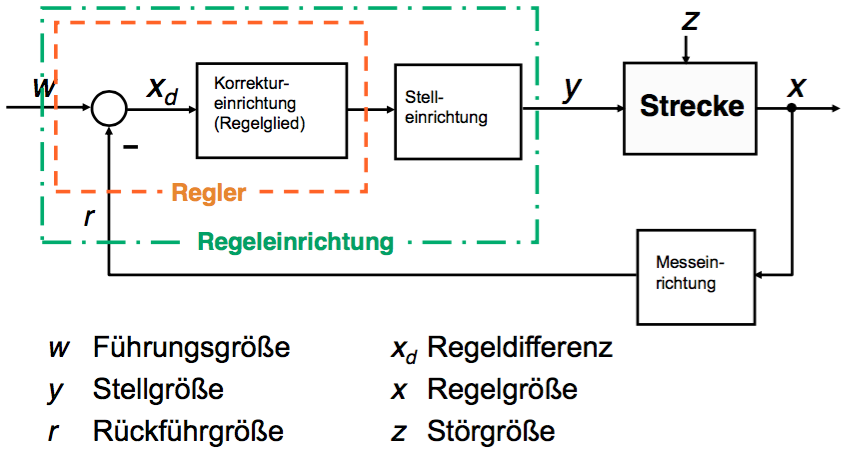
\includegraphics [scale=0.5]{regelkreis}
    \caption{Struktur eines Regelkreises}
\end{figure}

\mparagraph{Wirkungsweise}
\textbf{z} wird größer $\Rightarrow$ \textbf{x} wird gesenkt $\Rightarrow$ \textbf{r} wird abgesenkt
$\Rightarrow$ \textbf{$x_d$} wird angehoben $\Rightarrow$ \textbf{y} wird angehoben $\Rightarrow$
\textbf{x} wird angehoben mit der Tendenz den Sollwert \textbf{$x_s$} wieder anzunehmen. \\
Die Störgröße wird ausgeregelt.

\section{Grundlagen}
\subsection{Laplace Transformation}
\begin{compactitem}
    \item Rechenvereinfachung: Differential und Integralausdrücke werden zu algebraischen Ausdrücken.
    \item Gleichungslösung im Frequenzbereich statt Zeitbereich
    \item Integral muss konvergieren $\rightarrow$ lineare $f(t)$
\end{compactitem}
\begin{displaymath}
     L[f(t)] = f(s) = \int_0^\infty f(t)e^{-st}dt, s := \sigma + j\omega \text{ in } C \text{  } f(t)
      = 0, t < 0
\end{displaymath}

\begin{compactitem}
    \item \textbf{Linearitätssatz}: $L[\alpha f_i(t) + \beta f_2(t)] = \alpha f_1(s) + \beta f_2(s)$
    \item \textbf{Faltungssatz}: $L[f_1(t) * f_2(t)] = f_1(s) * f_2(s)$
    \item \textbf{Grenzwertsatz}: $f_1(t = 0) = \lim_{s \rightarrow \infty} s * f(s)$
    \item \textbf{Differentiationssatz}: $L[\frac{d}{dt}f(t)] = sF(s)$
    \item \textbf{Integrationssatz}: $L[\int f(t)dt] = \frac{1}{s}F(s)$

\end{compactitem}
\subsection{Übertragungsglieder}
\begin{compactitem}
    \item \textbf{P-Glied}: $y(t) = K * u(t)$
    \item \textbf{I-Glied}: $y(t) = K * \int_0^t u(\tau)d\tau$
    \item \textbf{D-Glied}: $y(t) = K * \dot{u}(t)$
    \item \textbf{T$_t$-Glied}: $y(t) = K * u(t-T_t)$
    \item \textbf{S-Glied}: $y(t) = K * \pm u_1(t) \pm u_2(t)$
    \item \textbf{KL-Glied}: $y(t) = K * F(u(t))$
    \item \textbf{M-Glied}: $y(t) = K * u_1(t)u_2(t)$
\end{compactitem}

\section{Reglertypen}
\subsection{PID Regler (und Unterklassen)}
\textbf{Sehr verbreitet, da für nahezu alle Prozesstypen geeignet, robust und mit geringem Aufwand
realisierbar} \\
P: güngstiges Regelverhalten, I: stationäre Genauigkeit, D: schnelle Ausregelung
\begin{align}
    u(t) = K_p (e(t) + \frac{1}{T_N}\int_o^t e(\tau)d\tau)+ T_V \frac{d}{dt}e(t))
\end{align}
mit Nachstellzeit $T_N$ und Vorhaltzeit $T_V$.

\mparagraph{Laplacetransformation}
\begin{align}
    u(t) &= K_Pe(t) + K_I \int e(t)dt + K_D \frac{d}{dt}e(t) \Leftrightarrow \\
    \Leftrightarrow u(s) &= K_Pe(s) + K_I \frac{1}{s}e(s) + K_Dse(s) \\
    \leftrightarrow \frac{u(s)}{e(s)} &= G(s) = K_P + K_I \frac{1}{s}+K_Ds \\
    \frac{\text{Ausgang}}{\text{Eingang}} &= \text{Übertragungsfunktion}
\end{align}
\subsection{Kennlinien- bzw. Kennlinienfeldregler}
\textbf{nihctlineare Übertragungsglieder}\\
z.B Zweipunktregler (Temperatur-Regelung)
\newpage
\subsection{Zustandsregler}
\textbf{Verbessertes Regelverhalten, da nicht nur die Regelabweichung, sondern im Idealfall alle
Zustandsgrößen der Regelstrecke zur Verfügung gestellt werden.} \\
regelungstechnische Behandlung von Mehrgrößensystemen, nichtlinearen und zeitvariablen
Übertragungssystemen.

\begin{figure}[!h]
    \centering
    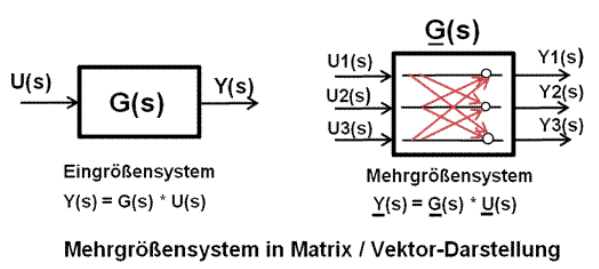
\includegraphics [scale=0.5]{mehrgroesse}
\end{figure}

\subsection{Kaskadenregelung}
\textbf{Unabhängige lineare Einzelregelkreis der einzelnen Gelenke}\\
Manipulator = Mehrgrößensystem

\begin{figure}[!h]
    \centering
    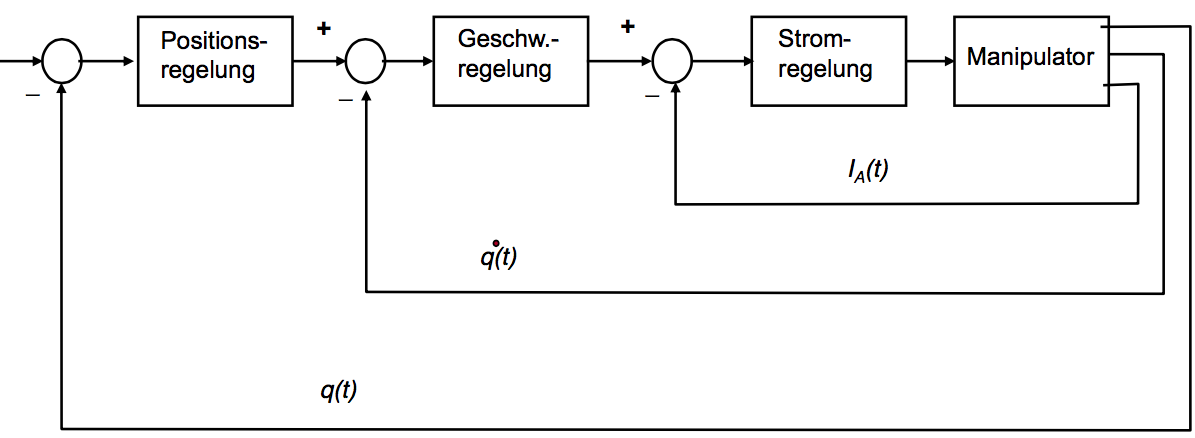
\includegraphics [scale=0.3]{kaskade}
\end{figure}

\subsection{Adaptive Regelung}
\textbf{Lageabhängige und somit zeitveränderliche Systemteile werden als Parameterschwankungen
aufgefasst}
\begin{figure}[!h]
    \centering
    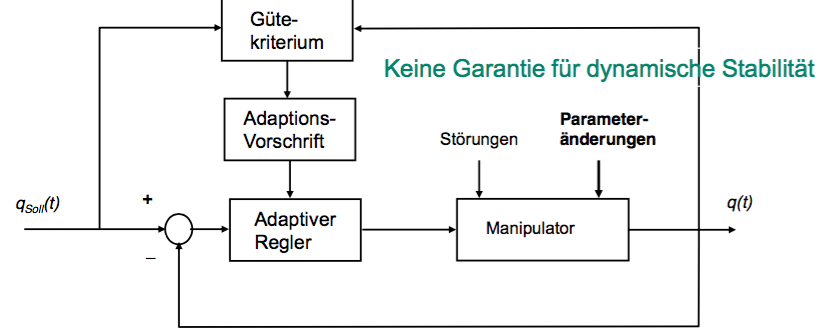
\includegraphics [scale=0.3]{adaptiv}
\end{figure}

\section{Regelungskonzepte für Manipulatoren}
\textbf{Regelung von Manipulatoren beschreibt nicht nur Positionsregelung, sondern auch die
Einbeziehung weiterer Umwelteinflüsste} (Massenträgheit des Manipulators, Gravitations-, Zentrifugal-,
Coriolis und Reibungskräfte/Momente auf die Gelenke)
\subsection{Exakte Systemmodellierung}
setzt a priori die exakte Kenntnis des Dynamikmodells und er Umgebung des Roboters voraus.
\subsection{Kraft-/Positionsregelung}
Position und Kräfte sind eng miteinander verknüpft. Steht Roboter in Kontakt mit Umgebung so bedeutet
Positionsänderung auch Kraftänderung und vice versa.

\mparagraph{Hybride Kraft-/Positionsregelung}
Wahlweise zwischen reiner Kraft und reiner Positionsregelung gewählt für jede kartesische Bewegungsrichtung
des Arms.
\mparagraph{Impedanz Regelung}
Regelt die dynamische Beziehung zwischen Kraft und Positions im Kontaktfall. \\
Idee: Interaktion Roboter-Umwelt verhält sich wie Feder-Dämpfer-Masse-System.
\begin{align}
     f(t) &= d * x(t)b * \dot{x}(t) + m * \ddot{x}(t)\\
     &\Rightarrow \text{Lapace Transformation} \Rightarrow \\
     F(s) &= (d + b+ s+ m *s ^2) * X(s)
\end{align}
Impedanz kann über Steifheit d, Dämpfung b und Trägheit m beeinflusst werden.

% !TEX root = rob1.tex
\chapter{Bahnsteuerung}

% !TEX root = rob1.tex
\chapter{Bahnplanung}

\section{Problemklassen}
\begin{itemize}
    \item \textbf{Klasse a)}
    \begin{compactitem}
        \item bekannt: vollständiges Umweltmodell und vollst. Neben-, Rand- und Zwangsbedingungen
        \item gesucht: Kollisionsfreie Bahn von Start zu Zielzustand
    \end{compactitem}
    \item \textbf{Klasse b)}
    \begin{compactitem}
        \item bekannt: unvollständiges Umweltmodell unvollst. Neben-, Rand- und Zwangsbedingungen
        \item gesucht: Kollisionsfreie Bahn von Start zu Ziel
        \item Problem: Kollision mit unbekannten Objekten
    \end{compactitem}
    \item \textbf{Klasse c)}
    \begin{compactitem}
        \item bekannt: zeitinvariantes Umweltmodell (bewegliche Hindernisse)
        \item gesucht: Kollisionsfreie Bahn von Start zu Zielzustand
        \item Problem: Hindernisse in Ort und Zeit variant
    \end{compactitem}
    \item \textbf{Klasse d)}
    \begin{compactitem}
        \item bekannt: kein Umweltmodell
        \item gesucht: Kollisionsfreie Bahn von Start zu Zielzustand
        \item Problem: Kartografie
    \end{compactitem}
    \item \textbf{Klasse e)}
    \begin{compactitem}
        \item bekannt: zeitvariantes Umweltmodell
        \item gesucht: Bahn zu einem beweglichen Ziel (Rendezvous Problem)
        \item Problem: Zielzustand in Ort und Zeit beweglich
    \end{compactitem}
\end{itemize}
\section{Definitionen}
\mparagraph{Umweltmodellierung}
\begin{compactitem}
    \item \textbf{Exakt}:Beispiel für constructed solid geometry, in Form einer
    algebraischen Beschreibung
    \item \textbf{Approximiert}: Die Umwelt wird duch Näherungen beschreiben (
    Kuben, verallgem. Zylinder, Polyeder)
\end{compactitem}

\mparagraph{Planungsalgorithmen}
\begin{compactitem}
    \item \textbf{Vollständige Verfahren}: Algorithmen liefern immer einer korrekte
    Lösung und können ermitteln, ob keine Lösung existiert
    \item \textbf{Probabilistische vollständige Verfahren}: Falls eine Lösung
    existiert konvergieren die Wahrscheinlichkeiten, dass eine Lösung gefunden
    wird bei fortschreitender Zeit gegen 1. Existiert keine Lösung, kann dies nicht
    ermittelt werden.
\end{compactitem}
\mparagraph{Konfiguration}
Eine Konfiguration q beschreibt den Zustand eines Roboters A im eukl. Raum durch Lage und Orientierung
oder im Gelenkwinkelzustandsraum durch die Werte der Gelenke.
\mparagraph{Konfigurationsraum}
Konfigurationsraum $C$ des Roboters A ist der Raum aller möglichen Konfigurationen von A
\mparagraph{Weg}
Weg für Roboter A von der Konfiguration q$_\text{Start}$ zur Konfiguration q$_\text{Ziel}$ ist eine
stetige Abbildung $\tau:[0,1] \rightarrow C$
\mparagraph{Arbeitsraumhindernis}
Arbeitsraumhindernis H ist der Raum, welcher von einem Objekt im Arbeitsraum eingenommen wird
\mparagraph{Konfigurationsraumhindernis}
$C_H$ ist die Menge aller Punkte des Konfigurationsraum, welche zu einer Kollision mit dem Hindernis
H führen
\mparagraph{Hindernisraum}
Menge aller Konfigurationsraumhindernisse $C_\text{obst} = \cup C_{H_i}$
\mparagraph{Freiraum}
Menge aller Punkte aus C, welche nicht im Hindernisraum liegen.
$C_\text{free} =  \{ q \in C | q \notin C_\text{obst}\} = C \backslash C_\text{obst}$

\section{Planungsverfahren}
\subsection{Mobile Roboter}
\begin{compactitem}
    \item Voronoi Diagramm
    \item Sichtgraph $\rightarrow$ Erweiterung der Hindernisse durch Kreis/Rechteck
    \item Zellenzerlegung
    \begin{compactitem}
        \item Exakte
        \item Approximative (Quad Tree)
    \end{compactitem}
    \item Potentialfelder mit Abstoßung und Anziehungspotentialen.
\end{compactitem}
\subsection{Manipulatoren}
\subsubsection{Probabilistic Roadmaps, PRM}
\begin{compactitem}
    \item Approximation des Freiraumes
\end{compactitem}
\begin{compactenum}
    \item Vorverarbeitung
    \begin{compactitem}
        \item Zufällige Erzeugung von kollisionsfreien Stichproben
        \item Stichproben werden über kollisionsfreien Pfad verbunden
    \end{compactitem}
    \item Anfrage
    \begin{compactitem}
        \item Verbinde Start und Ziel mit Wegnetz
        \item Suche im Graphen
    \end{compactitem}
\end{compactenum}

\subsubsection{Rapidly-exploring Random Tree}
\begin{compactitem}
    \item Algorithmus zur Einmalanfrage (keine Vorverarbeitung nötig)
    \item Aufbau zweier Bäume zur Approximatin des Freiraumes
\end{compactitem}

\begin{algorithm}[H]
    \begin{algorithmic}
        \State BUILD\_RRT(K$_\text{Start},n,\epsilon$)
        \State T.init(K$_\text{Start}$) Neuer Baum mit Startkonfiguration in der Wurzel
        \For {k=1 to n}
        \State K$_\text{Zuf} \leftarrow$ RAND\_CONF() Gleichverteilt zufällige Erzeugung einer Konfiguration
        \State K$_\text{Nahe} \leftarrow$ NEAREST\_VERTEX(K$_\text{Zuf}$, T) Bestimmung des nächsten Knoten
        \State K$_\text{Neu} \leftarrow$EXTEND(K$_\text{Nahe}$, K$_\text{Zuf}$, $\epsilon$) Erzeuge neue Konfiguration mit Abstand $\epsilon$ zu K$_\text{Nahe}$
        \State Falls Konfigurations gültig, füge neuen Knoten und Kante hinzu
        \EndFor
        \caption{RRT - Einfach}
    \end{algorithmic}
\end{algorithm}

\begin{algorithm}[H]
    \begin{algorithmic}
        \State 1. Aufbau von zwei Bäumen $T_1$ und $T_2$ mit Wurzelknoten $K_\text{Start}$ bzw. $K_\text{Ziel}$
        \State 2. Stichprobe K$_\text{Zuf}$ wird zur Erweiterung von $T_1$ verwendet mit Ergebni K$_\text{Neu}$
        \State 3. Erweiterung von $T_2$ mit K$_\text{Neu}$ bis K$_\text{Neu}$ erreicht oder !Valid(K$_\text{Neu}$)
        \State 4. Falls K$_\text{Neu}$ von $T_2$ erreicht wird, ist ein gültiger Pfad gefunden
        \State 5. Sonst: Vertausche Rolle von $T_1$ und $T_2$

        \caption{RRT - Bidirektional}
    \end{algorithmic}
\end{algorithm}

\textbf{Die Wahrscheinlichkeit, dass ein Knoten erweitert wird, ist proportional zur Größe der
entsprechenden Voronoi-Region}

\subsubsection{Glättung}
\begin{compactitem}
    \item Zufällige Wahl zweier Knoten im Lösungsweg
    \item Falls Verbindung kollisionsfrei, Verbinde beide Knoten und lösche dazwischenliegende Knoten
    aus dem Lösungspfad
\end{compactitem}

\subsubsection{Constrained Motion Planning}
\begin{compactitem}
    \item RRT Erweiterung
    \item VALID(K) unzureichend für Einschränkungen mit P(VALID(K))=0
    \item Erweiterung durch Berechnung von Distanz und/oder Richtung zu Konfiguration im Freiraum
    \item Ersetzung der Extend-Funktion
    \begin{compactitem}
        \item Randomized Gradient Descend
        \item First Order Retraction
    \end{compactitem}
\end{compactitem}

% !TEX root = rob1.tex
\chapter{Greifplanung}

\begin{figure}[!h]
    \centering
    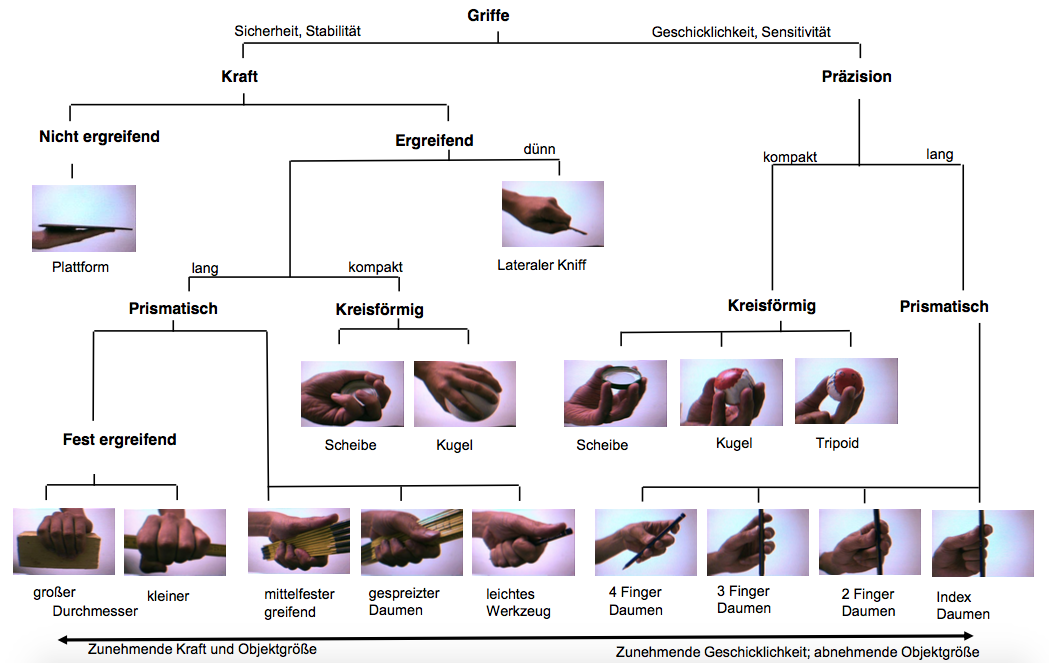
\includegraphics [scale=0.5]{griff}
    \caption{Cutkosky Grifftaxonomie}
\end{figure}

\section{Nebenbedinungen}
\subsection{Intern}
\begin{compactitem}
    \item \textbf{I1: Gültigkeit des Griffes}, Überlappung zwischen den Greifmerkmalen des zu greifenden
    Objektes und den Greifmerkmalen der Greiferfinger
    \item \textbf{I2: Kollisionsfreiheit des Griffes}, keine Kollision zwischen Greifer und gegriffenem
    Objekt
    \item \textbf{I3: Zugänglichkeit des Griffes}, der Griff ist für den Greifer kollisionsfrei erreichbar
\end{compactitem}
\subsection{Extern}
\begin{compactitem}
    \item \textbf{E1: Kollisionsfreie Anrückbewegung des Greifers}, keine Kollision zwischen Roboterarm,
    Grifer, benachbarten Objekten und Arbeitsebene
    \item \textbf{E2: Kollisionsfreie Abrückbewegung mit gegriffenem Objekt}, siehe e1
    \item \textbf{E3: Berücksichtigung der Roboterkinematik}, der selektierte Griff liegt im Arbeitsraum
    des Roboters und die korrespondierenden Trajektorien der Anrück und Abrückbewegung können
    können vom Roboter abgefahren werden.
    \item \textbf{E4: Stabilität des Griffes}, sowohl während der Greifbewegung der Greiferfinger als
    auch während der Transferbewegung des Greifers mit gegriffenem Objekt verändert sich die relative
    Lage und Orientierung des zu greifenden/gegriffenen Objekts zum Greifer nicht
    \item \textbf{E5: Stabilität der Szene}, Abrückbewegung des Greifers mit gegriffenem Objekt sollte
    die Stabilität der Szene nicht beeinflussen.
    \item \textbf{E6: Aufgabenabhängigkeit des Griffs}, wird Pick and Place Operation ausgeführt, dann
    muss zur Aufnahme und Ablagekonfiguration des zu greifenden Objektes kompatibler Griff gewählt werden.
    \begin{compactitem}
        \item Kann kein Griff bestimmt werden, der Nebenbedingung erfüllt, muss geeignete Umgreifsequenz
        bestimmt werden.
        \item Erfordert Griff Ausübung von Kraft und Kraftmomenten auf das Objekt, so muss Greifer diese
        Aufbringen können
    \end{compactitem}
\end{compactitem}

\section{Greifanalyse und Synthese}
\mparagraph{Greifanalyse}
\begin{compactitem}
    \item gegeben: Objekt und Menge von Kontaktpunkten
    \item gesucht: Aussagen zur Stabilität des Giffs unter Berücksichtung der Nebenbedinungen.
\end{compactitem}
\mparagraph{Greifsynthese}
\begin{compactitem}
    \item gegeben: Objekt und eine Menge von Nebenbedinungen.
    \item gesucht: Menge von Kontaktpunkten
\end{compactitem}

\section{Kontaktmodelle}
\begin{compactitem}
    \item Kontakt ohne Reibung (existiert nicht)
    \item Kontakt mit Reibung (Kraft wirkt normal als auch tangential zur Fläche)
    \item Soft-Kontakt (Kraft wirkt normal, tangential. Zusätzlich wirken axiale Momente)
\end{compactitem}
Reibungskegel wird kontinuierlich oder mit approximiert mit Polyeder beschrieben

\mparagraph{Wrenchvektor}
Vektor $\vec{w}$ fasst die in einem Kontaktpunkt $\vec{p}_i$ wirkenden Kräfte $f_i$ und Momente
$\tau_i$ mit $i \in \{x,y,z\}$ zusammen. \\
In Abhängigekeit vom Typ des i-ten Kontaktpunktes normalen \textbf{n}, tangentiale Kräft \textbf{t} und
axiale Momente \textbf{$\Theta$}: $^i\vec{w}_n, ^i\vec{w}_t, ^i\vec{w}_\Theta$ bzw. korrespondierende
Skalare $^ic_n, ^ic_t, ^ic_\Theta$
\mparagraph{Greifmatrix}
Darstellung der Wrenchvektoren für einen räumlichen Griff als Spaltenvektor einer 6 x 3m Matrix G.

\mparagraph{Gleichgewichtsgriff}
Ein Griff wird als Gleichgewichtsgriff bezeichne,t wenn die Summer aller Kräfte $f_i$ und Momente
$\tau_i$, die auf das gegriffene Objekt wirken, gleich Null ist.
\begin{align}
    &1. \forall i \in \{1, ...,m\} : ^ic_n \geq 0, ^i\mu_t * ^ic_n \geq |^ic_t|, ^i\mu_\Theta * ^ic_n
    \geq |^ic_\Theta| \\
    &2. \exists \vec{c} \in R^{3m}, \vec{c} \neq \vec{0} : G.\vec{c} + \vec{e} = 0
\end{align}
$^i\mu_t, ^i\mu_\Theta \in R$ = Coulombschen Reibungskoeffizienten am i-ten Kontaktpunkt

\section{Kraft und Formgeschlossene Griffe}




\end{document}
